\documentclass[12pt,a4paper]{article}

% ─── Page Layout ───────────────────────────────────────────────────────────────
\usepackage[a4paper, margin=0.8in, headheight=14pt]{geometry}

% ─── Fonts (XeLaTeX) ───────────────────────────────────────────────────────────
\usepackage{fontspec}
\usepackage{unicode-math}
\setmainfont{TeX Gyre Pagella}
\setmonofont[Scale=0.88]{TeX Gyre Cursor}
\setmathfont{Latin Modern Math}

% ─── Packages ──────────────────────────────────────────────────────────────────
\usepackage{xcolor}
\usepackage{colortbl}
\usepackage{titlesec}
\usepackage{enumitem}
\usepackage{tabularx}
\usepackage{booktabs}
\usepackage{array}
\usepackage{amsmath}
\usepackage{tikz}
\usetikzlibrary{shapes.geometric, arrows.meta, positioning, calc, fit, decorations.pathreplacing}
\usepackage{tcolorbox}
\tcbuselibrary{skins, breakable}
\usepackage{hyperref}
\usepackage{fancyhdr}
\usepackage{graphicx}
\usepackage{microtype}
\hyphenpenalty=10000
\exhyphenpenalty=10000
\sloppy
\usepackage{caption}
\usepackage{setspace}
\usepackage{multirow}
\usepackage{tocloft}

% ─── Q&A helper ────────────────────────────────────────────────────────────────
\newcommand{\Q}[1]{\textbf{#1}\par\noindent\ignorespaces}

% ─── Colour Palette ────────────────────────────────────────────────────────────
\definecolor{myred}{RGB}{196,30,58}
\definecolor{mydark}{RGB}{30,30,50}
\definecolor{mygreen}{RGB}{14,120,80}
\definecolor{myteal}{RGB}{0,130,140}
\definecolor{myamber}{RGB}{180,100,0}
\definecolor{mypurple}{RGB}{100,30,160}
\definecolor{mygray}{RGB}{246,247,249}
\definecolor{mgframe}{RGB}{180,185,200}
\definecolor{watermark}{RGB}{145,150,170}
\definecolor{hdrred}{RGB}{250,232,235}
\definecolor{hdrgreen}{RGB}{220,244,233}
\definecolor{hdrteal}{RGB}{220,242,244}
\definecolor{hdramber}{RGB}{253,242,215}
\definecolor{hdrpurple}{RGB}{238,228,255}
\definecolor{hdrgray}{RGB}{238,240,245}
\definecolor{rowalt}{RGB}{250,251,253}

% ─── Section Formatting ────────────────────────────────────────────────────────
\titleformat{\section}
  {\large\bfseries\color{myred}}{\thesection.}{0.5em}{}
  [\vspace{1pt}{\color{myred}\rule{\linewidth}{0.8pt}}]
\titleformat{\subsection}
  {\normalsize\bfseries\color{myteal}}{\thesubsection}{0.5em}{}
\titlespacing*{\section}{0pt}{18pt}{7pt}
\titlespacing*{\subsection}{0pt}{11pt}{4pt}

% ─── Paragraph ─────────────────────────────────────────────────────────────────
\setlength{\parindent}{0pt}
\setlength{\parskip}{4pt}

% ─── TOC Styling ───────────────────────────────────────────────────────────────
\renewcommand{\cfttoctitlefont}{\large\bfseries\color{myred}}
\renewcommand{\cftaftertoctitle}{\par\noindent{\color{myred}\rule{\linewidth}{0.8pt}}}
\setlength{\cftbeforetoctitleskip}{0pt}
\setlength{\cftaftertoctitleskip}{6pt}
\renewcommand{\cftsecfont}{\normalsize\bfseries\color{mydark}}
\renewcommand{\cftsecpagefont}{\normalsize\bfseries\color{mydark}}
\renewcommand{\cftsecleader}{\cftdotfill{\cftdotsep}}
\setlength{\cftbeforesecskip}{7pt}
\renewcommand{\cftsubsecfont}{\small\color{mydark}}
\renewcommand{\cftsubsecpagefont}{\small\color{mydark}}
\setlength{\cftbeforesubsecskip}{3pt}
\setlength{\cftsubsecindent}{1.4em}

% ─── Table helpers ─────────────────────────────────────────────────────────────
\renewcommand{\arraystretch}{1.45}
\setlength{\tabcolsep}{6pt}
\arrayrulecolor{mydark}
\newcolumntype{B}[1]{>{\small\bfseries\raggedright\arraybackslash}m{#1}}
\newcolumntype{Y}{>{\small\raggedright\arraybackslash}X}
\renewcommand{\tabularxcolumn}[1]{m{#1}}

% ─── Header / Footer ───────────────────────────────────────────────────────────
\pagestyle{fancy}
\fancyhf{}
\fancyhead[L]{\small\color{myred}\textbf{PE-EC603A}\;\color{mydark}--- Introduction to MEMS}
\fancyhead[R]{\small\color{myteal}\textbf{Module 3 Notes}}
\fancyfoot[C]{\small\color{mydark}\thepage}
\fancyfoot[R]{\small\color{watermark}\textit{\copyright\ Biraj}}
\renewcommand{\headrulewidth}{0.5pt}
\renewcommand{\footrulewidth}{0.3pt}

% ─── Hyperref ──────────────────────────────────────────────────────────────────
\hypersetup{
  colorlinks=true, linkcolor=myteal, urlcolor=myteal,
  pdfauthor={Biraj Sarkar},
  pdftitle={PE-EC603A --- Module 3 Notes}
}

% ─── tcolorbox styles ──────────────────────────────────────────────────────────
\tcbset{
  tikzbox/.style={
    colback=mygray, colframe=mgframe, boxrule=0.6pt, arc=4pt,
    left=8pt, right=8pt, top=6pt, bottom=6pt,
    colbacktitle=mgframe, coltitle=mydark,
    fonttitle=\small\bfseries
  },
  defbox/.style={
    colback=hdrgreen, colframe=mygreen, boxrule=0.8pt, arc=4pt,
    left=9pt, right=9pt, top=6pt, bottom=6pt,
    colbacktitle=mygreen, coltitle=white,
    fonttitle=\small\bfseries
  },
  formulabox/.style={
    colback=hdrteal, colframe=myteal, boxrule=0.8pt, arc=4pt,
    left=9pt, right=9pt, top=7pt, bottom=7pt,
    colbacktitle=myteal, coltitle=white,
    fonttitle=\small\bfseries
  },
  examplebox/.style={
    colback=hdramber, colframe=myamber, boxrule=0.8pt, arc=4pt,
    left=9pt, right=9pt, top=6pt, bottom=6pt,
    colbacktitle=myamber, coltitle=white,
    fonttitle=\small\bfseries
  },
  masonbox/.style={
    colback=hdrpurple, colframe=mypurple, boxrule=0.8pt, arc=4pt,
    left=9pt, right=9pt, top=6pt, bottom=6pt,
    colbacktitle=mypurple, coltitle=white,
    fonttitle=\small\bfseries
  },
  exambox/.style={
    colback=hdrpurple, colframe=mypurple, boxrule=1pt, arc=5pt,
    left=10pt, right=10pt, top=8pt, bottom=8pt,
    colbacktitle=mypurple, coltitle=white,
    fonttitle=\bfseries,
    breakable, title after break={\textbf{Frequently Asked / Viva Questions (contd.)}}}
}
% Make all boxes breakable across pages
\tcbset{breakable}

% ─── TikZ styles ───────────────────────────────────────────────────────────────
\tikzset{
  block/.style={rectangle, draw=myteal, fill=hdrteal,
    text width=2.4cm, align=center, minimum height=0.95cm,
    font=\small, rounded corners=3pt, line width=0.7pt},
  redblock/.style={rectangle, draw=myred, fill=hdrred,
    text width=2.4cm, align=center, minimum height=0.95cm,
    font=\small, rounded corners=3pt, line width=0.7pt},
  netnode/.style={rectangle, draw=myteal, fill=hdrteal,
    text width=1.5cm, align=center, minimum height=0.8cm,
    font=\small, rounded corners=3pt, line width=0.7pt},
  sumjunc/.style={circle, draw=myamber, fill=hdramber,
    minimum size=0.62cm, font=\small, line width=0.8pt},
  snode/.style={circle, draw=mypurple, fill=hdrpurple,
    minimum size=0.55cm, font=\footnotesize, line width=0.7pt},
  arrow/.style={-Stealth, thick, color=mydark},
  redarrow/.style={-Stealth, thick, color=myred},
  line/.style={thick, color=mydark}
}

% ═══════════════════════════════════════════════════════════════════════════════
\begin{document}
% ═══════════════════════════════════════════════════════════════════════════════

\begin{center}
  {\LARGE\bfseries\color{myred} PE-EC603A --- Introduction to MEMS}\\[5pt]
  {\normalsize\color{mydark} Semester VI \quad$\bullet$\quad 3L:0T:0P \quad$\bullet$\quad 3 Credits}\\[3pt]
  {\normalsize\color{myteal}\textbf{Module 3 Exam Notes: Sensors, Actuators \& Fabrication}}\\[3pt]
  {\small\color{mydark} CGEC \;$|$\; B.Tech ECE (2023--27) \;$|$\; \textit{Biraj Sarkar}}
\end{center}
\vspace{2pt}
\noindent{\color{myred}\rule{\linewidth}{1.5pt}}
\vspace{2pt}

\hypersetup{linkcolor=mydark}
\tableofcontents
\hypersetup{linkcolor=myteal}
\newpage

% ===============================================================================
\section{MEMS Sensors}
% ===============================================================================

Sensors are transduction elements that convert mechanical, thermal, optical, chemical, or biological signals from the physical environment into electrical outputs.

\subsection{Piezoresistive Sensors}
Piezoresistivity is the change in electrical resistivity ($\rho$) of a material when subjected to mechanical strain.
\begin{tcolorbox}[defbox]
\textbf{Gauge Factor ($G$):} The ratio of fractional change in resistance to the mechanical strain ($\epsilon$):
$$G = \frac{\Delta R / R}{\epsilon} = (1 + 2\nu) + \frac{\Delta\rho/\rho}{\epsilon}$$
where $\nu$ is the Poisson's ratio, and $\epsilon$ is the longitudinal strain.
\end{tcolorbox}
In metals, piezoresistivity is primarily due to geometric changes ($1+2\nu \approx 1.6$). In semiconductors like Silicon, it is dominated by band-structure changes under stress ($\Delta\rho/\rho \gg 1+2\nu$), yielding much higher gauge factors ($G \approx 100$ to $200$).

\textbf{Advantages:} High sensitivity, linear response, simple circuitry (Wheatstone bridge interface). \\
\textbf{Disadvantages:} Highly temperature-sensitive (requires compensation), drift over time.

\subsection{Capacitive Sensors}
Capacitive sensors measure changes in capacitance between a moving electrode and a fixed electrode:
$$C = \frac{\epsilon_r \epsilon_0 A}{d}$$

There are two primary modes of capacitive sensing:
\begin{itemize}[leftmargin=*, itemsep=4pt]
  \item \textbf{Gap-closing mode ($d$ changes):}
  $$C(x) = \frac{\epsilon_r \epsilon_0 A}{d_0 - x} \implies \frac{dC}{dx} = \frac{\epsilon_r \epsilon_0 A}{(d_0 - x)^2} \quad \text{(Non-linear, highly sensitive)}$$
  \item \textbf{Overlap-area mode ($A$ changes):}
  $$C(x) = \frac{\epsilon_r \epsilon_0 w (L - x)}{d} \implies \frac{dC}{dx} = -\frac{\epsilon_r \epsilon_0 w}{d} \quad \text{(Strictly linear)}$$
\end{itemize}

\textbf{Advantages:} Low power consumption, high temperature stability, negligible mechanical loading, low noise. \\
\textbf{Disadvantages:} Susceptible to electromagnetic interference (EMI) and parasitic capacitance (requires on-chip electronics).

\subsection{Piezoelectric Sensors}
Piezoelectric materials generate a transient surface charge $Q$ in response to applied force $F$:
$$Q = d_{ij} \cdot F$$
where $d_{ij}$ is the piezoelectric charge coefficient ($C/N$). Common materials include Quartz, Zinc Oxide ($ZnO$), Lead Zirconate Titanate ($PZT$), and Aluminum Nitride ($AlN$).

\textbf{Key Characteristic:} Active/self-generating sensor. It can only measure dynamic changes because static charges leak away through the measurement circuitry.

% ===============================================================================
\section{MEMS Actuators}
% ===============================================================================

Actuators convert electrical energy into mechanical movement or force.

\subsection{Electrostatic Comb Drive Actuators}
Comb drives consist of two interdigitated finger electrodes: one anchored (fixed) and one suspended on a spring (movable).

\begin{tcolorbox}[formulabox, title={Comb Drive Lateral Actuation Force}]
When a voltage $V$ is applied, the lateral force $F_x$ pulling the fingers together is:
$$F_x = N \frac{\epsilon_0 \epsilon_r h}{d} V^2$$
where:
\begin{tabular}{lcl}
$N$ & = & number of finger pairs \\
$h$ & = & thickness (height) of the fingers \\
$d$ & = & gap distance between the interdigitated fingers \\
$V$ & = & applied voltage
\end{tabular}
\end{tcolorbox}

\textbf{Crucial Feature:} The force $F_x$ is independent of lateral displacement $x$. This provides a stable, predictable force over a large range of motion, unlike parallel-plate electrostatic actuators (which suffer from pull-in instability).

\subsection{Thermal Actuators}
Thermal actuators utilize electrical resistive heating (Joule heating, $P = I^2 R$) to produce thermal expansion and generate mechanical movement.

\subsubsection{Thermal Bimorph}
Consists of two bonded layers with different Coefficients of Thermal Expansion ($\text{CTE}_1 > \text{CTE}_2$). Upon heating, the bimorph bends toward the material with the lower CTE (Layer 2).

\subsubsection{Chevron / V-Beam Actuator}
Symmetrical angled silicon beams anchored at the ends. Passing current through the beams causes thermal expansion, which forces the center shuttle forward in a linear direction, magnifying the displacement.

\subsection{Piezoelectric Actuators}
Piezoelectric actuators use the converse piezoelectric effect: applying an electric field $E$ induces mechanical strain $\epsilon = d_{ij} \cdot E$.
\begin{itemize}[leftmargin=*]
  \item \textbf{Stack Actuators:} Multiple thin piezoelectric layers stacked together.
  \item \textbf{Performance:} Extremely high force output, sub-nanometer resolution, but very small displacement (typically $< 0.1\%$ of length).
\end{itemize}

% ===============================================================================
\section{Microfabrication Processes}
% ===============================================================================

MEMS fabrication relies on modifying planar IC manufacturing steps for three-dimensional mechanical structures.

\subsection{Thermal Oxidation \& The Deal-Grove Model}
Thermal oxidation grows Silicon Dioxide ($SiO_2$) on Silicon at high temperatures ($900^{\circ}\text{C}$--$1200^{\circ}\text{C}$).
\begin{itemize}[leftmargin=*, itemsep=3.5pt]
  \item \textbf{Dry Oxidation ($Si + O_2 \to SiO_2$):} Slow growth rate, dense oxide, high dielectric strength. Used for electrical isolation.
  \item \textbf{Wet Oxidation ($Si + 2H_2O \to SiO_2 + 2H_2$):} Fast growth rate, less dense. Used as thick sacrificial layers.
\end{itemize}

\begin{tcolorbox}[defbox, title={The Deal-Grove Model}]
The Deal-Grove model describes the kinetics of thermal oxidation:
$$x_0^2 + A x_0 = B(t + \tau)$$
where $x_0$ is the oxide thickness, $t$ is oxidation time, $B$ is the parabolic rate constant, $B/A$ is the linear rate constant, and $\tau$ is a time shift parameter representing any pre-existing oxide layer.
\end{tcolorbox}

We identify two limiting regimes of the Deal-Grove model:
\begin{enumerate}[leftmargin=*, label=\arabic*., itemsep=3.5pt]
  \item \textbf{Reaction-limited (Linear) Regime (for short times, $t \ll \frac{A^2}{4B}$):}
  Here, $A x_0 \approx B(t + \tau) \implies x_0 \approx \frac{B}{A}(t + \tau)$.
  Oxide growth is limited by the rate of chemical reaction at the $Si$--$SiO_2$ interface.
  \item \textbf{Diffusion-limited (Parabolic) Regime (for long times, $t \gg \frac{A^2}{4B}$):}
  Here, $x_0^2 \approx B t \implies x_0 \approx \sqrt{B t}$.
  Oxide growth is limited by the rate of oxygen diffusing through the already grown oxide layer to reach the Silicon substrate.
\end{enumerate}

\subsection{Deposition Techniques}
\begin{itemize}[leftmargin=*, itemsep=4pt]
  \item \textbf{PVD (Physical Vapor Deposition):}
    \begin{itemize}[leftmargin=*, itemsep=2pt]
      \item \textbf{Thermal Evaporation:} Heating a target material in high vacuum until it evaporates and condenses on the substrate.
      \item \textbf{Sputtering:} Bombarding a target material with heavy inert gas ions ($Ar^+$) in a plasma, ejecting target atoms toward the substrate.
    \end{itemize}
  \item \textbf{CVD (Chemical Vapor Deposition):} Gases react chemically at the substrate surface to deposit a thin film.
    \begin{itemize}[leftmargin=*, itemsep=2pt]
      \item \textbf{LPCVD (Low Pressure CVD):} High temperature ($> 600^{\circ}\text{C}$), high film purity and uniformity. Used to deposit Polysilicon and Silicon Nitride ($Si_3N_4$).
      \item \textbf{PECVD (Plasma Enhanced CVD):} Plasma assists the reaction, allowing low temperature deposition ($200^{\circ}\text{C}$--$400^{\circ}\text{C}$). Used to deposit dielectrics over metal layers.
    \end{itemize}
\end{itemize}

\subsection{Photolithography Process Flow}
Photolithography transfers geometric patterns from a photo-mask to a light-sensitive polymer (photoresist) on the substrate:
\begin{enumerate}[leftmargin=*, label=\arabic*., itemsep=2.5pt]
  \item \textbf{Substrate Preparation:} Clean wafer and apply adhesion promoter (HMDS).
  \item \textbf{Spin Coating:} Spin liquid photoresist at high speed to obtain a uniform thin film.
  \item \textbf{Soft Bake:} Heat wafer ($90^{\circ}\text{C}$--$100^{\circ}\text{C}$) to evaporate solvents and stabilize resist.
  \item \textbf{Alignment and Exposure:} Align mask to wafer and expose to ultraviolet (UV) light.
  \item \textbf{Development:} Immerse wafer in chemical developer to dissolve selective resist regions.
  \item \textbf{Hard Bake:} Heat wafer ($110^{\circ}\text{C}$--$130^{\circ}\text{C}$) to polymerize and harden the remaining resist.
\end{enumerate}

\textbf{Positive vs. Negative Photoresist:}\par\noindent
\begin{tabularx}{\linewidth}{|B{3.2cm}|Y|Y|}
\hline
\textbf{Property} & \textbf{\color{myteal}Positive Photoresist} & \textbf{\color{mygreen}Negative Photoresist} \\
\hline
\textbf{UV Exposure Effect} & Exposed area becomes soluble in developer. & Exposed area polymerizes/cross-links, becoming insoluble. \\
\hline
\textbf{Mask Pattern Copy} & Identical to mask pattern. & Reversal of mask pattern. \\
\hline
\textbf{Resolution} & Extremely high (sub-micron). & Lower (swelling occurs during development). \\
\hline
\textbf{Common Material} & DNQ-Novolac. & SU-8, polyisoprene-based. \\
\hline
\end{tabularx}

\subsection{Etching and LIGA}
\begin{itemize}[leftmargin=*, itemsep=3.5pt]
  \item \textbf{Wet vs. Dry:} Wet etching uses liquid chemicals (high selectivity, isotropic). Dry etching uses gas plasmas (high anisotropy).
  \item \textbf{Isotropic vs. Anisotropic:} Isotropic etches equally in all directions (creates undercuts). Anisotropic etches in a preferred direction (vertical walls).
  \item \textbf{LIGA:} A German acronym for Lithographie, Galvanoformung, Abformung (Lithography, Electroplating, Molding). Uses synchrotron X-ray source to fabricate metal/plastic components with extremely high aspect ratios ($>100:1$).
\end{itemize}

% ===============================================================================
\section{Surface Micromachining and Stiction}
% ===============================================================================

Surface micromachining builds micro-structures on top of the substrate by depositing and patterning alternating structural and sacrificial layers.

\subsection{Release Etch Sequence}
The most common surface micromachining process uses Silicon as the substrate, Silicon Dioxide ($SiO_2$) as the sacrificial layer, and Polysilicon as the structural material. The sacrificial oxide is removed using hydrofluoric acid (HF) to release the moving polysilicon structures.

\begin{tcolorbox}[tikzbox, title={Surface Micromachining Cantilever Release Sequence}]
\centering
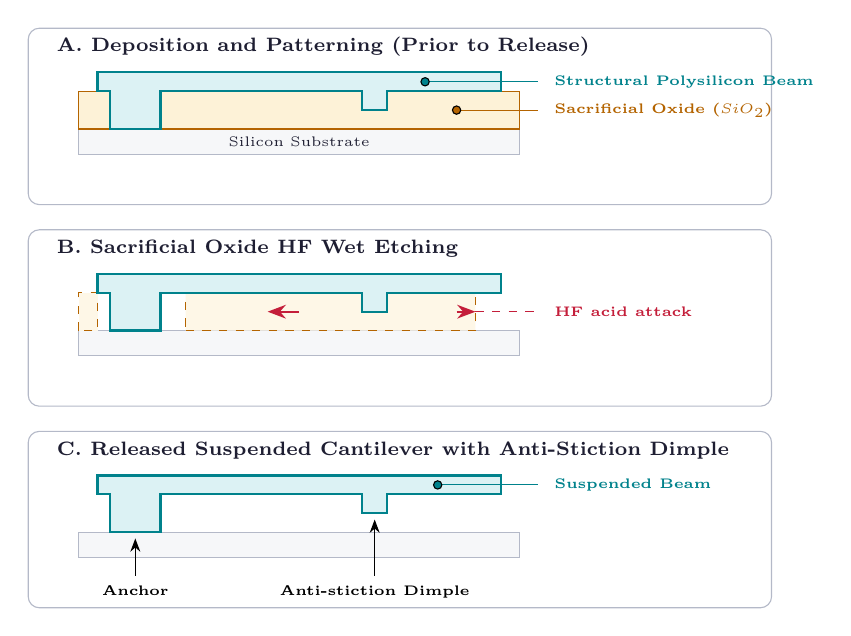
\begin{tikzpicture}[x=0.8cm, y=0.8cm, >=Stealth]
  % STATE 1: Prior to Release
  \begin{scope}[shift={(0,6.4)}]
    \draw[fill=white, draw=mgframe, rounded corners=4pt] (-0.3,-1.2) rectangle (11.5,1.6);
    \node[anchor=west, font=\scriptsize\bfseries\color{mydark}] at (0,1.3) {A. Deposition and Patterning (Prior to Release)};
    % Substrate
    \draw[fill=mygray, draw=mgframe] (0.5,-0.4) rectangle (7.5,0);
    \node[font=\tiny, color=mydark] at (4,-0.2) {Silicon Substrate};
    % Sacrificial Oxide
    \draw[fill=hdramber, draw=myamber] (0.5,0) rectangle (1.0,0.6);
    \draw[fill=hdramber, draw=myamber] (1.8,0) -- (7.5,0) -- (7.5,0.6) -- (5.4,0.6) -- (5.4,0.3) -- (5.0,0.3) -- (5.0,0.6) -- (1.8,0.6) -- cycle;
    % Structural Poly-Si
    \draw[fill=hdrteal, draw=myteal, thick] (0.8,0.6) -- (1.0,0.6) -- (1.0,0) -- (1.8,0) -- (1.8,0.6) -- (5.0,0.6) -- (5.0,0.3) -- (5.4,0.3) -- (5.4,0.6) -- (7.2,0.6) -- (7.2,0.9) -- (0.8,0.9) -- cycle;
    
    % Horizontal Leader Lines and Labels on the right side
    \draw[myteal, thin] (6.0,0.75) -- (7.8,0.75);
    \draw[fill=myteal] (6.0,0.75) circle (1.5pt);
    \node[anchor=west, font=\tiny\bfseries, color=myteal] at (7.9,0.75) {Structural Polysilicon Beam};
    
    \draw[myamber, thin] (6.5,0.3) -- (7.8,0.3);
    \draw[fill=myamber] (6.5,0.3) circle (1.5pt);
    \node[anchor=west, font=\tiny\bfseries, color=myamber] at (7.9,0.3) {Sacrificial Oxide ($SiO_2$)};
  \end{scope}

  % STATE 2: Wet HF Etch Attack
  \begin{scope}[shift={(0,3.2)}]
    \draw[fill=white, draw=mgframe, rounded corners=4pt] (-0.3,-1.2) rectangle (11.5,1.6);
    \node[anchor=west, font=\scriptsize\bfseries\color{mydark}] at (0,1.3) {B. Sacrificial Oxide HF Wet Etching};
    % Substrate
    \draw[fill=mygray, draw=mgframe] (0.5,-0.4) rectangle (7.5,0);
    % Shrinking Oxide (represented with dashed boundaries)
    \draw[fill=hdramber!60, draw=myamber, dashed] (0.5,0) rectangle (0.8,0.6);
    \draw[fill=hdramber!60, draw=myamber, dashed] (2.2,0) -- (6.8,0) -- (6.8,0.6) -- (5.4,0.6) -- (5.4,0.3) -- (5.0,0.3) -- (5.0,0.6) -- (2.2,0.6) -- cycle;
    % Structural Poly-Si
    \draw[fill=hdrteal, draw=myteal, thick] (0.8,0.6) -- (1.0,0.6) -- (1.0,0) -- (1.8,0) -- (1.8,0.6) -- (5.0,0.6) -- (5.0,0.3) -- (5.4,0.3) -- (5.4,0.6) -- (7.2,0.6) -- (7.2,0.9) -- (0.8,0.9) -- cycle;
    % HF Etch arrows
    \draw[redarrow] (4,0.3) -- (3.5,0.3);
    \draw[redarrow] (6.5,0.3) -- (6.8,0.3);
    
    % Leader Line and Label for acid attack
    \draw[myred, thin, dashed] (6.8,0.3) -- (7.8,0.3);
    \node[anchor=west, font=\tiny\bfseries, color=myred] at (7.9,0.3) {HF acid attack};
  \end{scope}

  % STATE 3: Released Structure with Dimple
  \begin{scope}[shift={(0,0)}]
    \draw[fill=white, draw=mgframe, rounded corners=4pt] (-0.3,-1.2) rectangle (11.5,1.6);
    \node[anchor=west, font=\scriptsize\bfseries\color{mydark}] at (0,1.3) {C. Released Suspended Cantilever with Anti-Stiction Dimple};
    % Substrate
    \draw[fill=mygray, draw=mgframe] (0.5,-0.4) rectangle (7.5,0);
    % Structural Poly-Si (Oxide is completely gone)
    \draw[fill=hdrteal, draw=myteal, thick] (0.8,0.6) -- (1.0,0.6) -- (1.0,0) -- (1.8,0) -- (1.8,0.6) -- (5.0,0.6) -- (5.0,0.3) -- (5.4,0.3) -- (5.4,0.6) -- (7.2,0.6) -- (7.2,0.9) -- (0.8,0.9) -- cycle;
    
    % Leader Line and Label for suspended beam
    \draw[myteal, thin] (6.2,0.75) -- (7.8,0.75);
    \draw[fill=myteal] (6.2,0.75) circle (1.5pt);
    \node[anchor=west, font=\tiny\bfseries, color=myteal] at (7.9,0.75) {Suspended Beam};
    
    % Labels below the substrate (within card bounds)
    \draw[<-] (1.4,-0.1) -- (1.4,-0.7) node[below, font=\tiny\bfseries] {Anchor};
    \draw[<-] (5.2,0.2) -- (5.2,-0.7) node[below, font=\tiny\bfseries] {Anti-stiction Dimple};
  \end{scope}
\end{tikzpicture}
\end{tcolorbox}

\subsection{Release Stiction Mechanism}
During drying after wet HF etching, liquid water forms a meniscus between the suspended beam and the substrate.
\begin{enumerate}[leftmargin=*, label=\arabic*.]
  \item As the liquid evaporates, capillary forces (surface tension $F_s \propto L^1$) pull the compliant beam down.
  \item If the beam touches the substrate, solid-solid adhesion forces (van der Waals, hydrogen bonding, electrostatic charge) keep it permanently attached to the substrate. This is called \textbf{Stiction}.
\end{enumerate}

\subsection{Stiction Mitigation Techniques}
\begin{itemize}[leftmargin=*, itemsep=4pt]
  \item \textbf{Anti-stiction Dimples:} Small molded bumps on the underside of the beam (fabricated by etching small shallow pits in the sacrificial oxide prior to structural polysilicon deposition). Dimples reduce the physical contact area by $>98\%$ if the beam collapses, preventing stiction forces from bonding the surfaces.
  \item \textbf{Supercritical CO2 Drying (SCD):} The wet rinsing liquid is replaced with liquid carbon dioxide ($CO_2$). The temperature and pressure are raised above the supercritical point of $CO_2$ ($31.1^{\circ}\text{C}$, $73.9\text{ atm}$), transitioning it directly into gas without a liquid-vapor phase boundary. This completely eliminates surface tension forces, preventing cantilever collapse.
  \item \textbf{Dry Release Processes:} Replacing sacrificial oxide with a polymer layer that is released using an oxygen plasma dry ash, avoiding liquid contact entirely.
\end{itemize}

\newpage
% ===============================================================================
% MANDATORY QUICK REVISION PAGE
% ===============================================================================
\begin{center}
  {\large\bfseries\color{myred} Quick Revision --- Module III}\\[3pt]
  {\small\color{mydark} Sensors, Actuators \& Fabrication $|$ PE-EC603A}
\end{center}
\noindent{\color{myred}\rule{\linewidth}{1.2pt}}
\vspace{4pt}

\begin{tcolorbox}[formulabox, title={\textbf{Key Transduction Formulas}}]
\renewcommand{\arraystretch}{1.3}
\begin{tabularx}{\linewidth}{B{3.8cm} Y Y}
\textbf{Transduction Mechanism} & \textbf{Core Equation} & \textbf{Key Variable Definition} \\
\hline
Piezoresistive Sensitivity & $\displaystyle\frac{\Delta R}{R} = G \cdot \epsilon$ & $G$: Gauge Factor; $\epsilon$: Long strain \\[8pt]
Capacitive Sensitivity (Gap) & $\displaystyle\frac{dC}{dx} = \frac{\epsilon A}{(d_0 - x)^2}$ & $A$: Plate area; $d_0$: Initial gap \\[8pt]
Comb Drive Force (Lateral) & $\displaystyle F_x = N \frac{\epsilon_0 \epsilon_r h}{d} V^2$ & $N$: Finger pairs; $h$: thickness; $d$: gap \\[8pt]
Deal-Grove Kinetics & $x_0^2 + A x_0 = B(t + \tau)$ & $B$: Parabolic rate; $B/A$: Linear rate \\[2pt]
\end{tabularx}
\end{tcolorbox}

\begin{tcolorbox}[defbox, title={\textbf{One-Line Definitions}}]
\begin{itemize}[leftmargin=*, itemsep=2.5pt, topsep=0pt]
  \item \textbf{Gauge Factor ($G$):} The normalized sensitivity of a resistor to mechanical strain; $G_{\text{Silicon}} \gg G_{\text{Metal}}$.
  \item \textbf{Piezoelectric Effect:} The generation of electric charge in response to mechanical stress; utilized in high-frequency resonators.
  \item \textbf{Comb Drive:} An electrostatic actuator utilizing interdigitated fingers to produce constant lateral force.
  \item \textbf{Deal-Grove Model:} A kinetic theory modeling the thermal oxidation rate of silicon under linear and parabolic regimes.
  \item \textbf{Positive Photoresist:} A photo-sensitive polymer that becomes soluble in developer upon UV exposure (e.g., DNQ-Novolac).
  \item \textbf{LIGA:} A micromachining process combining X-ray lithography, electroplating, and molding for extreme aspect ratios.
  \item \textbf{Stiction:} The unwanted permanent adhesion of released micro-mechanical structures to the adjacent substrate.
  \item \textbf{Supercritical Drying:} A drying method eliminating capillary collapse by evaporating $CO_2$ above its supercritical point.
\end{itemize}
\end{tcolorbox}

\begin{tcolorbox}[exambox, title={\textbf{Frequently Asked / Viva Questions}}]
\begin{enumerate}[topsep=0pt, label=\textbf{Q\arabic*.}, itemsep=5pt]
  \item \Q{Why does Silicon exhibit a much higher Gauge Factor ($G$) than typical metals?}
    In metals, $G \approx 2$ is caused only by dimensional changes. In Silicon, $G \approx 100-200$ due to the piezoresistive effect, where mechanical strain changes the semiconductor band gap and mobility ($\rho$).
  \item \Q{Explain why a capacitive sensor is preferred over a piezoresistive sensor for low-power applications.}
    Capacitive sensors consume near-zero DC power because they act as open circuits to DC, whereas piezoresistive sensors require continuous current flow through a Wheatstone bridge.
  \item \Q{Derive why the lateral force in a comb drive actuator remains constant over displacement.}
    Since lateral capacitance $C(x) = 2N \frac{\epsilon h(x_0 + x)}{d}$, the energy $U = \frac{1}{2} C V^2$. The lateral force is $F_x = \frac{dU}{dx} = \frac{1}{2} \frac{dC}{dx} V^2 = N \frac{\epsilon h}{d} V^2$, which has no dependence on $x$.
  \item \Q{Contrast dry oxidation and wet oxidation in silicon processing.}
    Dry oxidation ($O_2$) is slow, producing a high-quality, dense oxide film. Wet oxidation ($H_2O$) is fast, producing a less dense oxide, ideal for thick sacrificial oxide spacers in MEMS.
  \item \Q{Identify the rate-limiting steps in the two regimes of the Deal-Grove model.}
    In the linear regime ($t \to 0$), growth is limited by the chemical reaction rate at the silicon interface. In the parabolic regime ($t \to \infty$), growth is limited by oxidant diffusion through the oxide layer.
  \item \Q{Detail the steps of the photolithography process flow.}
    Substrate clean $\to$ HMDS spin $\to$ Spin coat photoresist $\to$ Soft bake $\to$ Align and expose to UV $\to$ Develop $\to$ Hard bake.
  \item \Q{How does a positive photoresist differ from a negative photoresist?}
    Positive resist exposed to UV becomes soluble and is washed away. Negative resist exposed to UV cross-links, becomes insoluble, and remains, while unexposed resist is developed away.
  \item \Q{Describe the stiction problem and how dimples mitigate it.}
    Liquid water evaporation during release drying creates capillary forces that pull micro-beams down. Bonding forces keep them stuck. Dimples are tiny underside bumps that minimize contact area, preventing bonding.
  \item \Q{Why does Supercritical CO2 drying prevent the collapse of micro-cantilevers?}
    Supercritical drying heats and pressurizes $CO_2$ above its critical point, bypassing the liquid-gas boundary. This eliminates surface tension ($\gamma = 0$), preventing any capillary forces from pulling the beam down.
  \item \Q{What is LIGA and what is its primary advantage?}
    LIGA uses X-ray lithography, electroplating, and molding. It allows the fabrication of non-silicon (metal/plastic) micro-parts with extremely high aspect ratios ($>100:1$).
\end{enumerate}
\tcbset{breakable}
\end{tcolorbox}

\begin{tcolorbox}[tikzbox, title={Comparison: Etching Methods in MEMS}]
\renewcommand{\arraystretch}{1.45}
\par\noindent
\begin{tabularx}{\linewidth}{|B{3.2cm}|Y|Y|}
\hline
\textbf{Parameters} & \textbf{\color{myteal}Wet Chemical Etching} & \textbf{\color{mypurple}Dry Plasma Etching (DRIE)} \\
\hline
\textbf{Mechanism} & Liquid chemical reactant bath. & Gas-phase reactive ions / plasma bombardment. \\
\hline
\textbf{Selectivity} & Very High (excellent material selectivity). & Moderate. \\
\hline
\textbf{Directionality} & Isotropic (undercuts mask) or anisotropic along crystal planes (KOH). & High Anisotropy (produces vertical sidewalls). \\
\hline
\textbf{Etch Rate} & Fast. & Slow to moderate. \\
\hline
\textbf{Common Use} & Sacrificial release (HF), cavity etch (KOH). & High-aspect-ratio trench etch (Bosch process). \\
\hline
\end{tabularx}
\tcbset{breakable}
\end{tcolorbox}

\end{document}
